% \cleartorightpage\begin{savequote}[75mm]
% Genome annotation is like the CliffsNotes for the DNA manual of life. Without it, we're just flipping through the pages cluelessly. But with it, we can finally understand what the heck is going on inside our cells.
% \qauthor{ChatGPT}
% \end{savequote}


\chapter{In the Cell}\label{chapter:annotation}
\setcounter{figure}{-1}
\setcounter{table}{-1}
\setcounter{section}{-1}
%\setcounter{enumiv}{-1}
\setcounter{NAT@ctr}{-1}

% \begin{figure}[t!]
% 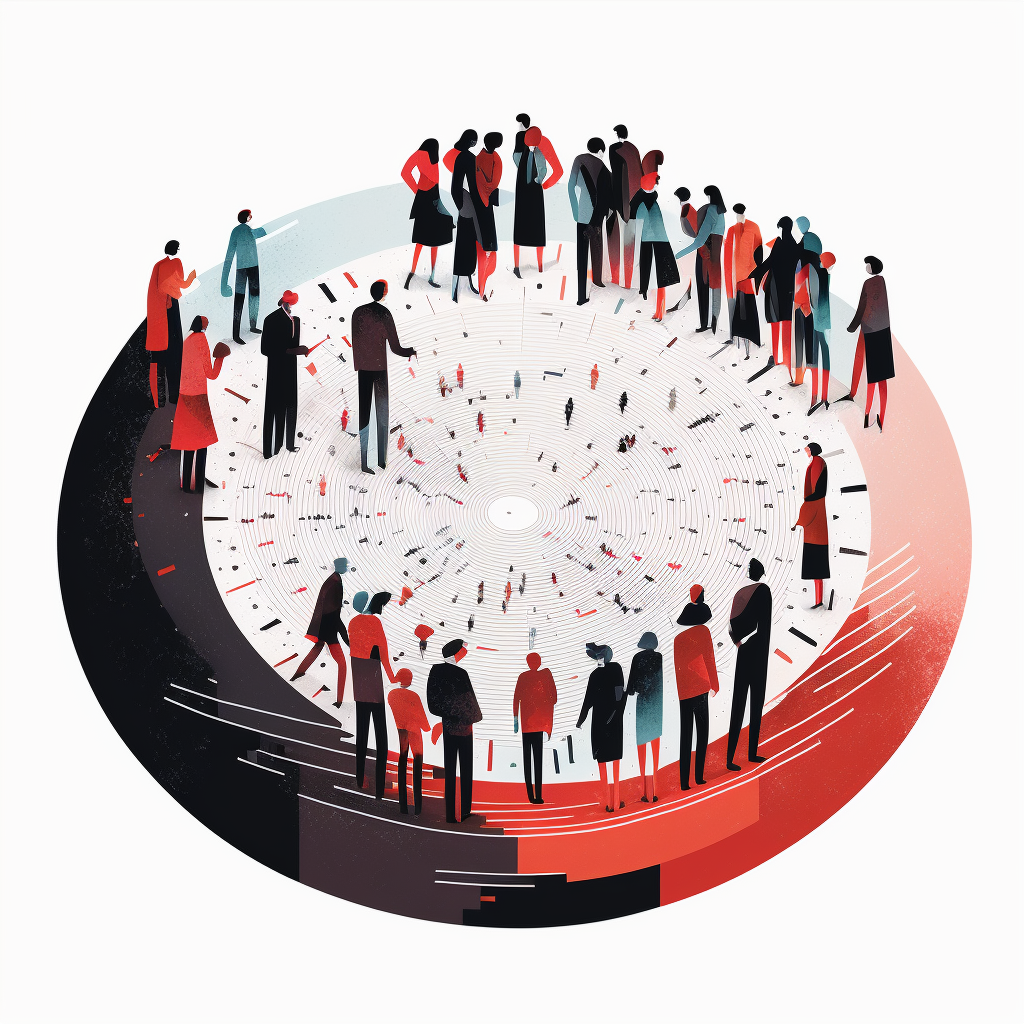
\includegraphics[height=10em]{chapters/header-annotation.png}
% \end{figure}
\setcounter{figure}{-1}
\setcounter{table}{-1}
\setcounter{section}{-1}

\lettrine[lines=3,lraise=0.30,lhang=0.3,findent=0.5em,nindent=0em]{\textcolor{hexy-red}{\fontEBGaramondInitials{}G}}{\color{hexy-red}enome annotation} is the cornerstone on which all modern genomics and bioinformatics research is built. Just DNA or RNA by itself is more or less meaningless for research, especially clinical research if we cannot tell which genes there, much less if they are up- or down-regulated. Manual annotation is extremely important for high quality results, as fully automatic annotation in genomics experiences a significant ``garbage in garbage out'' problem, as well as ``annotation drift'' where propagation of annotation is not always correct.

This chapter presents a series of tools centered around the Generic Model Organism Database (GMOD) community, a set of independent open-source projects which all interoperate to provide a scalable platform for genome annotation, from sequencing to publication. The concrete implementation of this suite for bacteriophage annotation is discussed which enables scaling of the limited number of human annotators and training of the next generation of annotators.
The combined power of the GMOD platform is then leveraged to enable an entire curriculum and phage annotation pipeline around these systems and interconnections. Additionally, a complex tool used in this field is given a new interface which is more easily accessible and reusable for a larger audience.

\begin{enumerate}[label=\ref*{chapter:annotation}.\arabic*]
\itemsep-0.5em
\setcounter{enumi}{-1}
\item \textbf{\color{hexy-red}Galaxy and Apollo as a biologist-friendly interface for high-quality cooperative phage genome annotation.} In this work we discuss the development of Galaxy and Apollo together to form a highly reproducible and interoperable annotation workbench that's accessible even to undergraduate students. I started the work (Python, XML, Docker) to make Galaxy and Apollo interoperable by developing numerous tools and bridges between the two services, before working together with other members of the Center for Phage Technology to scale this up into a production service beyond the needs of their phage annotation course. Additionally I was the original developer of many of the 50 new tools and wrappers for external software that are available from within Galaxy.

\item \textbf{\color{hexy-red}Galactic Circos: User-friendly creation of Circos Plots within the Galaxy platform.} Circos is an extremely popular tool for visualisation of high dimension and genome scale data, especially in publications and posters. But this generally requires an experienced bioinformatician to design, hand-code, and then hard-code the plot making it rather inflexible without experienced help. Saskia Hiltemann and I created a Galaxy port of Circos, allowing it to be essentially completely configurable via browser. Due to Circos' inherent complexity, this became probably the single most complex Galaxy tool wrapper. However, at these costs, it had additional positive interactions with Galaxy, as users could take their analysis results essentially directly into Circos, simplifying their workflows. We additionally wrote extensive training materials as part of the publication, in order to improve accessibility.

\end{enumerate}
